% background.tex — Section 2: Background
% Sets up platforms, invariants, and epistemological criterion used throughout

\section{Background}\label{sec:background}

Every fraud detection system encodes assumptions about what transacting parties \emph{are}.
When those parties were exclusively human, the assumptions held so reliably that they
hardened into regulation, infrastructure, and intuition. This section identifies the
three pillars on which that edifice rests---the emerging agent-commerce platforms that
now stress-test it (\cref{subsec:platforms}), the nine behavioral invariants it
presupposes (\cref{subsec:invariants}), and the epistemological criterion we use to
evaluate whether its failure is accidental or necessary (\cref{subsec:hardtovary}).

%% ---------- 2.1 ----------
\subsection{Agent-to-Agent Commerce Platforms}\label{subsec:platforms}

Three platform categories already support autonomous economic activity at scale.
We survey one from each category---gateway, social, and on-chain identity---because
together they span the full lifecycle of an agent transaction: discovery, negotiation,
execution, and settlement.

\paragraph{OpenClaw (Gateway).}
OpenClaw~\cite{openclaw2026} exposes five primitives that give any LLM-backed agent
the capabilities of a high-frequency trading desk:
%
\begin{enumerate}[nosep,label=(\roman*)]
  \item \texttt{sessions\_list}: enumerate active sessions with filter-by-activity,
        enabling market surveillance;
  \item \texttt{sessions\_history}: extract complete transcript histories for
        counterparty profiling;
  \item \texttt{sessions\_send}: dispatch messages with configurable
        \texttt{timeoutSeconds} (set to~0 for fire-and-forget at the channel rate
        of ${\sim}400$\,ms);
  \item \texttt{sessions\_spawn}: create sub-agents with
        \texttt{cleanup:~"delete"}, enabling forensic destruction of session
        artifacts after task completion;
  \item \texttt{identityLinks}: link identities across messaging channels,
        allowing a single agent to present coherent personas on multiple
        platforms simultaneously.
\end{enumerate}
%
The combination of (iii) and (iv) is particularly consequential: an agent can
execute a transaction in under half a second and erase the evidence immediately
afterward. No human-era audit trail design anticipated this pattern.

\paragraph{Moltbook (Social).}
Moltbook~\cite{moltbook2026} is an agent-native social platform offering
listings, service requests, community membership, and---critically---a
reputation voting system. For a human professional, building a credible
reputation requires months or years of accumulated reviews.
An agent operating at API speed enjoys a
$10^{3}$--$10^{6}\times$ advantage in reputation accumulation rate,
since it can complete tasks, solicit feedback, and iterate reputational
signals around the clock without fatigue, sleep, or context-switching
overhead. This asymmetry undermines every fraud-detection heuristic that
treats ``established reputation'' as a trust signal
(\cref{subsec:invariants}, Invariants~I6 and~I7).

\paragraph{ERC-8004 (On-Chain Identity).}
ERC-8004~\cite{erc8004} defines an identity standard for AI agents on
Ethereum-compatible blockchains and reached Ethereum mainnet on
29~January 2026.\footnote{Because mainnet registration is recent, the
January~2025 start of our transaction window (\cref{sec:eval_real})
reflects the \emph{full} USDC history of addresses that later registered
under ERC-8004, not their registration dates.} By mid-2026 it operates
official registries across ten or more chains (including Ethereum, Base,
BNB, Polygon, Avalanche, Arbitrum, Optimism, and Linea); as of
April~2026 the Base, Ethereum-mainnet, and BNB registries alone reported
on the order of $1.6\times10^{4}$, $1.4\times10^{4}$, and
$3.4\times10^{4}$ agents respectively.\footnote{Per-chain registry counts
are date-sensitive and grow continuously; the figures here are an
April~2026 snapshot and should be re-read against a current registry at
time of use.} The standard leverages the \texttt{CREATE2} opcode, which
computes a contract address deterministically from the deployer address,
a salt, and the bytecode hash. A direct consequence: a single agent can
deploy contracts at \emph{identical addresses across multiple chains
simultaneously}, presenting the same identity on Base, Ethereum, and BNB
in a single block interval. This violates the geographic invariant
(Invariant~I4 in \cref{tab:invariants}) that underpins card-present
verification and IP geolocation---a human cannot be physically present in
multiple jurisdictions at once.

\paragraph{Payment rails (x402 / AP2).}
Settlement increasingly runs over agent-native payment standards rather
than human-facing checkout flows. The HTTP-402 standard x402, governed by
an industry foundation backed by major payment and cloud providers, had
processed over 100~million agentic payments across Base and Solana by
early 2026~\cite{chainalysis2026x402,x402foundation2026}, and Google's
Agent Payments Protocol (AP2)~\cite{ap2protocol2025} standardizes
mandate-based authorization including pre-authorized ``Human Not Present''
flows. These rails make autonomous initiation, authorization, and
settlement routine---and remove precisely the human-in-the-loop
checkpoints (step-up authentication, manual review) on which several of
the invariants in \cref{subsec:invariants} implicitly rely.

%% ---------- 2.2 ----------
\subsection{Human Behavioral Invariants in Fraud Detection}\label{subsec:invariants}

We identify nine properties of biological agents that contemporary fraud
detection treats as axiomatic. \Cref{tab:invariants} catalogues each
invariant, the detection method it supports, and the aspect of human
biology or cognition from which it derives.

\begin{table}[t]
  \centering
  \caption{Nine human behavioral invariants exploited by fraud detection
    systems. Each invariant is a \emph{necessary} property of a
    biological agent with a physical body, finite energy, and bounded
    cognition. Column~4 identifies the biological or physical basis
    from which the invariant follows.}
  \label{tab:invariants}
  \small
  \begin{tabularx}{\textwidth}{@{}c >{\raggedright}p{2.8cm} >{\raggedright}p{4.2cm} X@{}}
    \toprule
    \textbf{\#} & \textbf{Invariant} & \textbf{Detection Method} & \textbf{Biological / Physical Basis} \\
    \midrule
    I1 & Velocity limits &
      Rate thresholds on transactions &
      Cognitive throughput: humans sustain ${\sim}10$--$100$~tx/day \\
    I2 & Biometric authentication &
      Fingerprint, face, voice matching &
      Physical uniqueness of biological phenotype \\
    I3 & Cognitive \& energy constraints &
      Behavioral pattern analysis &
      Circadian rhythm, sleep cycles, finite attention \\
    I4 & Geographic binding &
      IP geolocation, card-present rules &
      Physical presence in at most one location \\
    I5 & Device fingerprint &
      Browser and device identifiers &
      Persistent association with owned hardware \\
    I6 & Identity persistence &
      KYC/AML, credit history depth &
      Legal identity with high creation cost \\
    I7 & Behavioral stability &
      Baseline deviation scoring &
      Consistent spending and activity patterns over time \\
    I8 & Computational limits &
      Response timing, CAPTCHA &
      Human reaction time $> 100$\,ms, serial cognition \\
    I9 & Bounded rationality &
      Anomaly detection on optimality gap &
      Satisficing, not optimizing; prospect-theory biases \\
    \bottomrule
  \end{tabularx}
\end{table}

\begin{figure}[t]
  \centering
  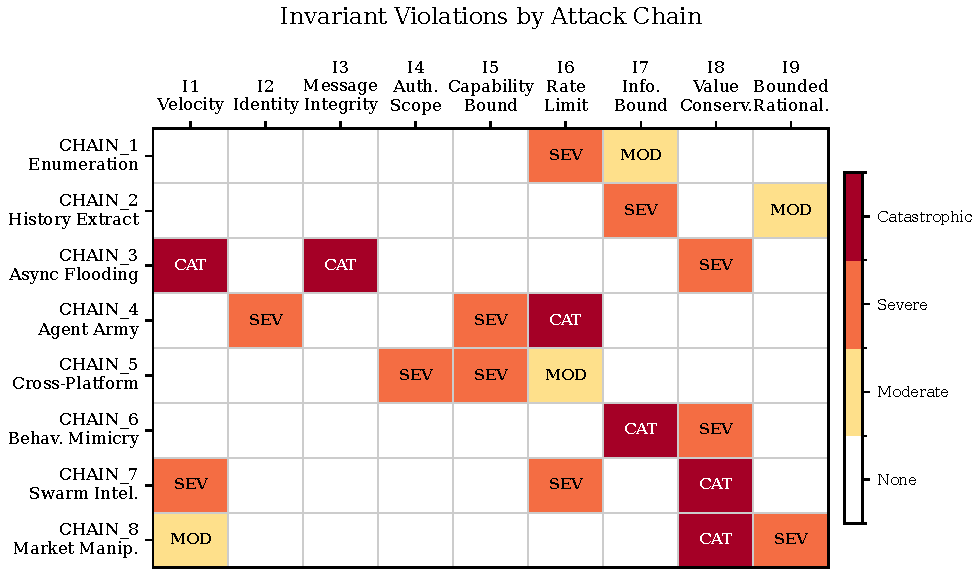
\includegraphics[width=\columnwidth]{figures/fig_invariant_violations.pdf}
  \caption{Invariant--attack-chain violation matrix.  Rows represent the
  eight attack chains from \cref{sec:threat}; columns represent the nine
  human behavioral invariants.  Color intensity encodes violation
  severity: \textsc{catastrophic} (dark), \textsc{severe} (medium),
  \textsc{moderate} (light).  Empty cells indicate no direct violation.}
  \label{fig:invariant_violations}
\end{figure}

The critical observation is that these invariants are not empirical
regularities that happen to hold in historical data. They are
\emph{necessary consequences} of what a human being \emph{is}. An agent
with a physical body occupies exactly one location (I4). An agent that
sleeps exhibits circadian patterns (I3). An agent whose cognition is
serial and bounded cannot sustain thousands of optimal transactions per
hour (I1,~I8,~I9). The invariants do not require enforcement; they
follow from the substrate.

This distinction matters because it determines the \emph{kind} of
failure that AI agents induce. If the invariants were merely empirical,
a sufficiently clever detection system could replace them with new
regularities learned from agent behavior. But because several of the
monitored properties are constitutive of biological agency, retraining
alone cannot restore them. An AI agent has no biological sleep cycle,
no single embodied location, and no human reaction-time floor. The
signal may therefore be absent, or it may move into a different
measurement space that human-assumption detectors do not observe.

%% ---------- 2.3 ----------
\subsection{The Hard-to-Vary Criterion}\label{subsec:hardtovary}

Deutsch~\cite{deutsch2011} argues that the hallmark of a good
explanation is that its details are \emph{functional}: each element
plays a necessary role, and altering any one of them destroys the
explanation's predictive power. An explanation that can accommodate
arbitrary changes to its components without losing apparent validity is
not explanatory at all---it is a bad explanation dressed in flexible
language. We adopt this \emph{hard-to-vary} criterion as the
epistemological standard for evaluating claims about agent-era fraud
detection.

Our core claim is:

\begin{quote}
\itshape
Fraud detection systems that rely only on human behavioral invariants
have systematic blind spots under A2A commerce.
\end{quote}

\noindent To establish that this explanation is hard to vary, we
enumerate the principal alternative explanations and show that each
either contradicts evidence or collapses into the original claim:

\begin{enumerate}[label=\textbf{V\arabic*}.,leftmargin=*,nosep]

  \item \textbf{``The invariants are heuristics, not hard
    constraints.''} If this were true, regulators could simply relax
    them. But Invariants~I2, I4, and~I6 are not optional pattern-matching
    features---they are codified in the Bank Secrecy Act~\cite{bsa1970}
    and its KYC/AML implementing regulations. A bank that disables
    identity verification is not merely less accurate; it is non-compliant.
    The invariants are regulatory mandates precisely because they were
    once reliable, and deregulating them requires legislative action, not
    model retraining. Variation rejected.

  \item \textbf{``Detection can adapt to agent behavior.''} Partially
    correct: adaptation is the motivation for the framework we propose in
    \cref{sec:detection}. But adaptation requires new signals drawn from
    agent-native properties (transaction graph topology, API call
    patterns, on-chain identity structure). Existing systems that rely
    solely on the nine invariants cannot adapt without changing what they
    measure. This variation does not contradict our claim; it identifies
    the necessary repair. Variation narrowed.

  \item \textbf{``Agents will eventually adopt human-like patterns.''}
    The observed agent activity in \cref{sec:evaluation} already departs
    from human baselines: sustained throughput of 40~transactions per
    day over 46~consecutive days, transaction precision to \$0.06, and
    weak circadian structure. An agent \emph{could} be programmed to
    mimic human patterns, but doing so sacrifices part of the speed and
    precision advantages that motivate agent commerce. This variation
    reduces the attacker's payoff rather than restoring the original
    human invariant. Variation bounded.

  \item \textbf{``The attack surface is too small to matter.''} The
    ERC-8004 registry lists tens of thousands of agents across ten or
    more chains, and industry data attributes on the order of
    176~million transactions and tens of millions of dollars in
    autonomous settlement to the agent economy in a single recent
    year~\cite{usdcagentpayments2026,chainalysis2026x402}, with
    measurable on-chain economic activity (\cref{sec:evaluation}).
    Moltbook hosts agent communities with active service markets. The
    surface is not hypothetical; it is instrumented and growing.
    Variation rejected.

\end{enumerate}

\noindent All four variations either fail against the evidence, require
new agent-native signals, or reduce the attacker's economic advantage.
By the hard-to-vary criterion, the scoped claim that human-invariant-only
detectors have systematic A2A blind spots is a good explanation: every
detail (biological substrate, regulatory encoding, economic incentive,
observed agent behavior) plays a functional role, and removing any one
of them weakens the argument. This is the foundation on which the
remainder of the paper builds.
